%%%%%%%%%%%%%%%%%%%%%%%%%%%%%%%%%%%%%%%%%
% Beamer Presentation
% LaTeX Template
% Version 1.0 (10/11/12)
%
% This template has been downloaded from:
% http://www.LaTeXTemplates.com
%
% License:
% CC BY-NC-SA 3.0 (http://creativecommons.org/licenses/by-nc-sa/3.0/)
%
%%%%%%%%%%%%%%%%%%%%%%%%%%%%%%%%%%%%%%%%%

%----------------------------------------------------------------------------------------
%	PACKAGES AND THEMES
%----------------------------------------------------------------------------------------

\documentclass{beamer}

\mode<presentation> {

% The Beamer class comes with a number of default slide themes
% which change the colors and layouts of slides. Below this is a list
% of all the themes, uncomment each in turn to see what they look like.

%\usetheme{default}
%\usetheme{AnnArbor}
%\usetheme{Antibes}
%\usetheme{Bergen}
%\usetheme{Berkeley}
%\usetheme{Berlin}
%\usetheme{Boadilla}%         +
%\usetheme{CambridgeUS}%     ++
%\usetheme{Copenhagen}
%\usetheme{Darmstadt}
%\usetheme{Dresden}
%\usetheme{Frankfurt}
%\usetheme{Goettingen}%        ++
%\usetheme{Hannover}  %        +
%\usetheme{Ilmenau}
%\usetheme{JuanLesPins}
%\usetheme{Luebeck}
%\usetheme{Madrid}
%\usetheme{Malmoe}
%\usetheme{Marburg}
%\usetheme{Montpellier}
%\usetheme{PaloAlto}
%\usetheme{Pittsburgh}
\usetheme{Rochester}
%\usetheme{Singapore}
%\usetheme{Szeged}        %        ++
%\usetheme{Warsaw}

% As well as themes, the Beamer class has a number of color themes
% for any slide theme. Uncomment each of these in turn to see how it
% changes the colors of your current slide theme.

%\usecolortheme{albatross}
\usecolortheme{beaver}
%\usecolortheme{beetle}
%\usecolortheme{crane}
%\usecolortheme{dolphin}
%\usecolortheme{dove}              % ++
%\usecolortheme{fly}
%\usecolortheme{lily}               % ++
%\usecolortheme{orchid}
%\usecolortheme{rose}
%\usecolortheme{seagull}
%\usecolortheme{seahorse}
%\usecolortheme{whale}
%\usecolortheme{wolverine}
%\usecolortheme{owl}

%\setbeamertemplate{footline} % To remove the footer line in all slides uncomment this line
%\setbeamertemplate{footline}[page number] % To replace the footer line in all slides with a simple slide count uncomment this line

%\setbeamertemplate{navigation symbols}{} % To remove the navigation symbols from the bottom of all slides uncomment this line
}

\usepackage{graphicx} % Allows including images
\usepackage{booktabs} % Allows the use of \toprule, \midrule and \bottomrule in tables
\usepackage[english,russian]{babel}
\usepackage{mathtools}

\addtobeamertemplate{navigation symbols}{}{%
	\usebeamerfont{footline}%
	\usebeamercolor[fg]{footline}%
	\hspace{1em}%
	\insertframenumber/\inserttotalframenumber
}

%------------------------------------------------
%	TITLE PAGE
%------------------------------------------------

\title[КР: Сжатие словарей для анализа исходных кодов]{
	КУРСОВАЯ РАБОТА\\ 
	Исследовательский проект \\
	``Сжатие словарей для нейросетевого анализа исходных кодов программ''
} % The short title appears at the bottom of every slide, the full title is only on the title page

\author{
	 Выполнил: Андрей Гусев \\
Руководитель КР: Чиркова Надежда Александровна
} % Your name
\institute[ПМИ ВШЭ] % Your institution as it will appear on the bottom of every slide, may be shorthand to save space
{
Высшая Школа Экономики\\ % Your institution for the title page
\medskip
\textit{aagusev\_2@edu.hse.ru} % Your email address
}
\date{\today} % Date, can be changed to a custom date

\begin{document}

\begin{frame}
\titlepage % Print the title page as the first slide
\end{frame}



%\begin{frame}
%\frametitle{Содержание} % Table of contents slide, comment this block out to remove it
%\tableofcontents % Throughout your presentation, if you choose to use \section{} and \subsection{} commands, these will automatically be printed on this slide as an overview of your presentation
%\end{frame}

%------------------------------------------------
%	PRESENTATION SLIDES
%------------------------------------------------

\begin{frame}
\frametitle{Прунинг входного слоя}
Матрица эмбеддингов $\mathsf E$ задает представление $L$ элементов словаря. Сумму рассматриваемых регуляризаторов $\mathrm R(\mathsf E)$ можно представить в следующем виде:

\[\mathrm R(\mathsf E) = 
\underbrace{\lambda_{1} \sum_{l=1}^{L} \|\mathsf E_l\|_2 }_\text{group Lasso}
+ 
\underbrace{\lambda_{2} \|\mathsf E\|_1 }_\text{
	Lasso}
, \text{ где $\|\cdot\|_2$ --- это $ \ell^2-$норма}
\]

Lasso-регуляризация стимулировует обнуление одного веса в строке, а group Lasso --- к последующему обнулению всей строки.
\end{frame}


%------------------------------------------------

\begin{frame}
\frametitle{Encoder Code2Seq}
\begin{figure}
	\centering
	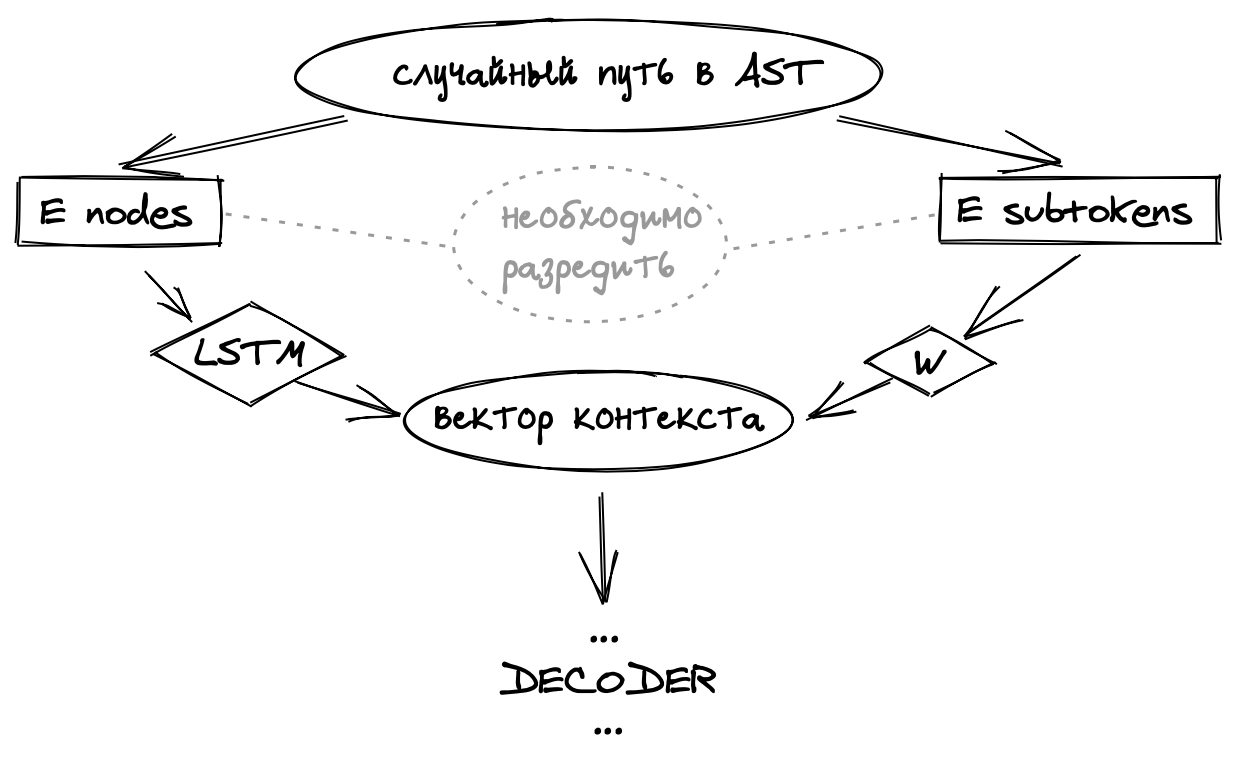
\includegraphics[width=0.8\textwidth]{graphics/c2s_encoder.png}
\end{figure}
\end{frame}

%------------------------------------------------

\begin{frame}
\frametitle{Сравнение с базовой моделью}
\begin{table}[htbp]
	\tiny
	\centering
	\begin{tabular}{lrrrr}
		\toprule
		{} &  $\mathsf{Val\ F1}$ & $\mathsf{Test\ F1}$ &  $\mathsf{nodes}$ & $\mathsf{subtokens}$\\
		\midrule
		\textbf{разреженная$^{1}$} &  0.4239 &  0.4195 & 177 & 10029\\
		\textbf{ограниченная$^{2}$} & 0.4201 & 0.4277& 177 & 10029 \\
		\textbf{оригинальная$^{3}$} & 0.4092 & 0.4229 & 323 & 73906\\
		\bottomrule
	\end{tabular}
\end{table}


{
	\footnotesize
	$\ ^1$Средние результаты трех запусков с предложенной техникой разреживания
	
	$\ ^2$Результаты запуска модели с простой техникой сжатия
	
	$\ ^3$Усредненные результаты исходной модели
}
\end{frame}


%------------------------------------------------


\end{document} 
